\section{Qualidade de Software}

A qualidade do \textit{software} é um aspecto fundamental que impacta diretamente a eficácia do sistema em seu contexto de uso \citeonline{iso25000}. A norma \citeonline{iso25000} define a qualidade do produto de \textit{software} em termos de características e subcaracterísticas que determinam sua capacidade de satisfazer as necessidades explícitas e implícitas dos usuários. Além disso, a qualidade em uso refere-se ao efeito percebido pelo usuário final ao interagir com o \textit{software} em seu ambiente operacional.

A avaliação da qualidade de um produto de \textit{software} em uso é essencial para garantir que o sistema não apenas funcione conforme especificado, mas também atenda às expectativas e requisitos dos usuários em situações reais de operação. As características e subcaracterísticas da qualidade em uso são definidas pela norma \citeonline{iso25010} e são apresentadas na Figura \ref{fig:quality-in-use}.

\begin{figure}[h]
\centering
\caption{Modelo de Qualidade em Uso}
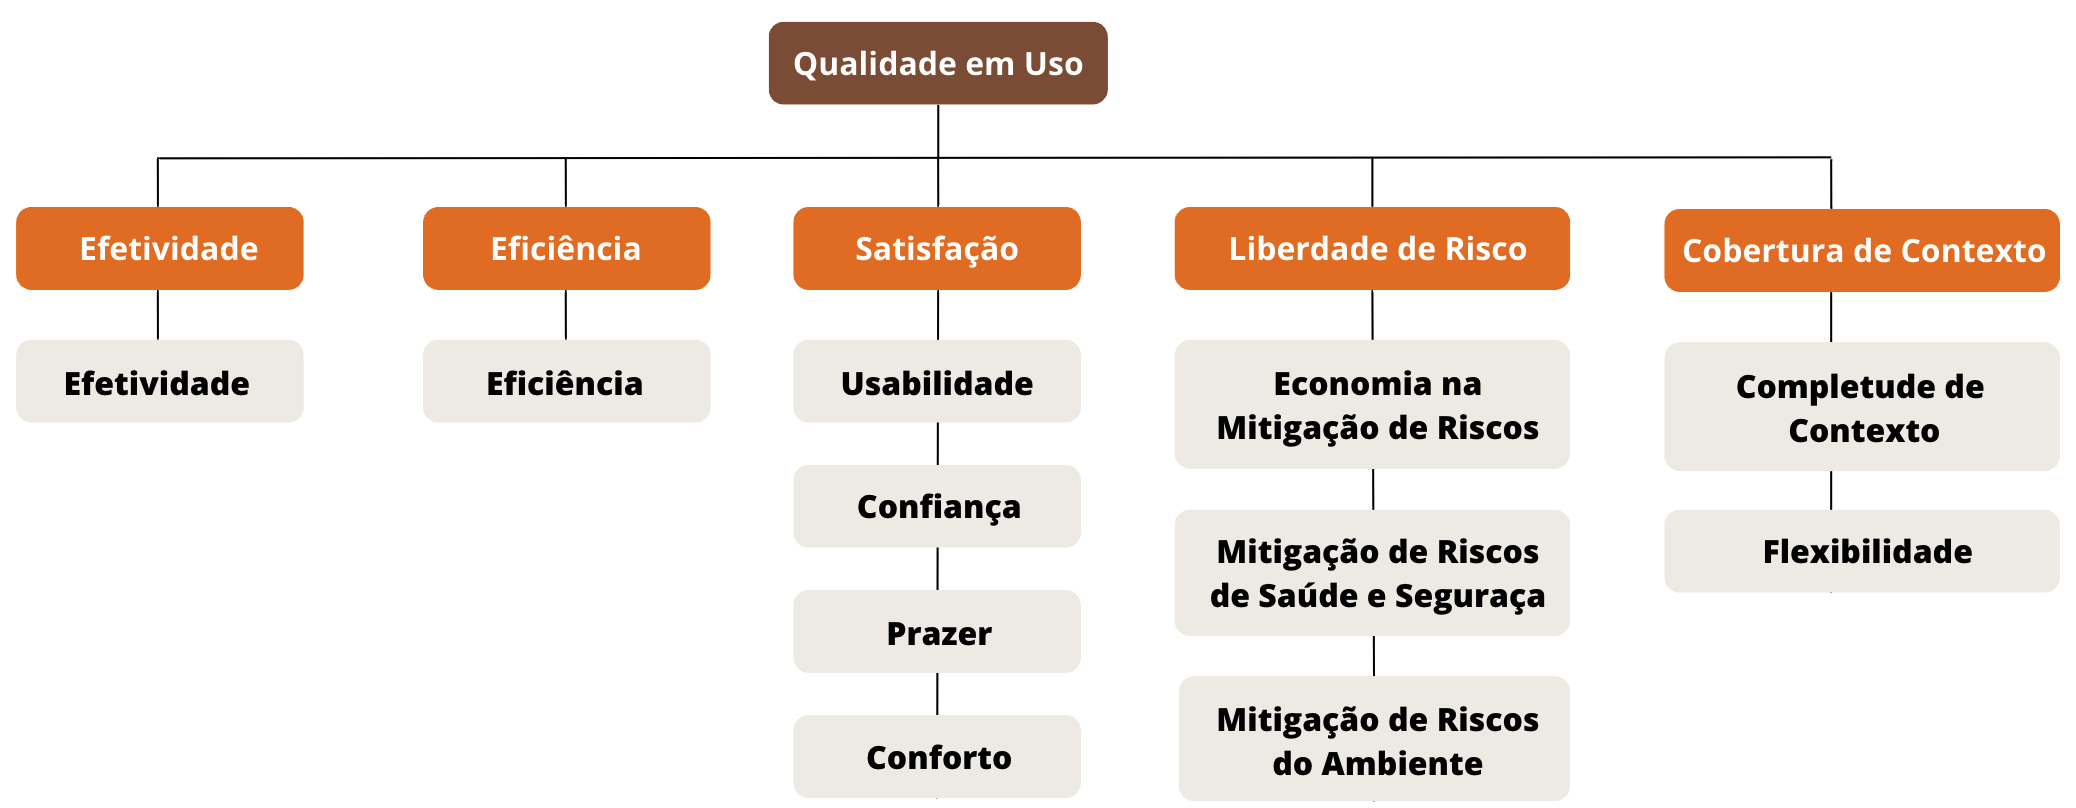
\includegraphics[width=1\linewidth]{figuras/quality_in_use.png}
\text{Fonte: Norma \citeonline{iso25010}}
\label{fig:quality-in-use}
\end{figure}

O foco desta monografia está na característica de qualidade de \textbf{eficácia}. A eficácia refere-se à precisão e à completude com que o \textit{software} permite que os usuários alcancem os objetivos esperados. A norma \citeonline{iso9241} define que, para avaliar determinada característica, devem ser definidas medidas de critério para tal, e exemplifica que, em termos de eficácia, estas devem estar relacionadas a quantidade de vezes que uma tarefa é realizada com sucesso, garantindo que o usuário alcançou seus objetivos específicos.

Os experimentos controlados visam, dentre outros objetivos, aumentar a qualidade do \textit{software}, entregando apenas as funcionalidades que realmente agregam valor para o usuário \cite{fabijan_online_2020}. As métricas observadas no momento de avaliar o tratamento em um experimento são escolhidas para validar se os usuários realmente preferem a nova versão, o que pode ser interpretado como nível de eficácia da variante.
